\subsection{Class Diagram}
The Class Diagram presented in the RASD document showed in a generic way the problem; instead, the following diagram has the objective to present the solution to that problem. For this reason, it is more implementation-oriented and detailed with respect to the one inserted in the RASD, and so it is more useful for developers. In particular, the following changes have been performed:
\begin{itemize}
	\item Introduction of the main methods of StoreManager and Customer classes.
	\item Introduction of the User class, which is a generalization of the two classes StoreManager and Customer.
	\item Introduction of the data type of the attributes.
	\item Removal of the NoTechCustomer class, since it was useful only for modelling the problem and not the solution.
\end{itemize}
\begin{figure}[H]
\centerline{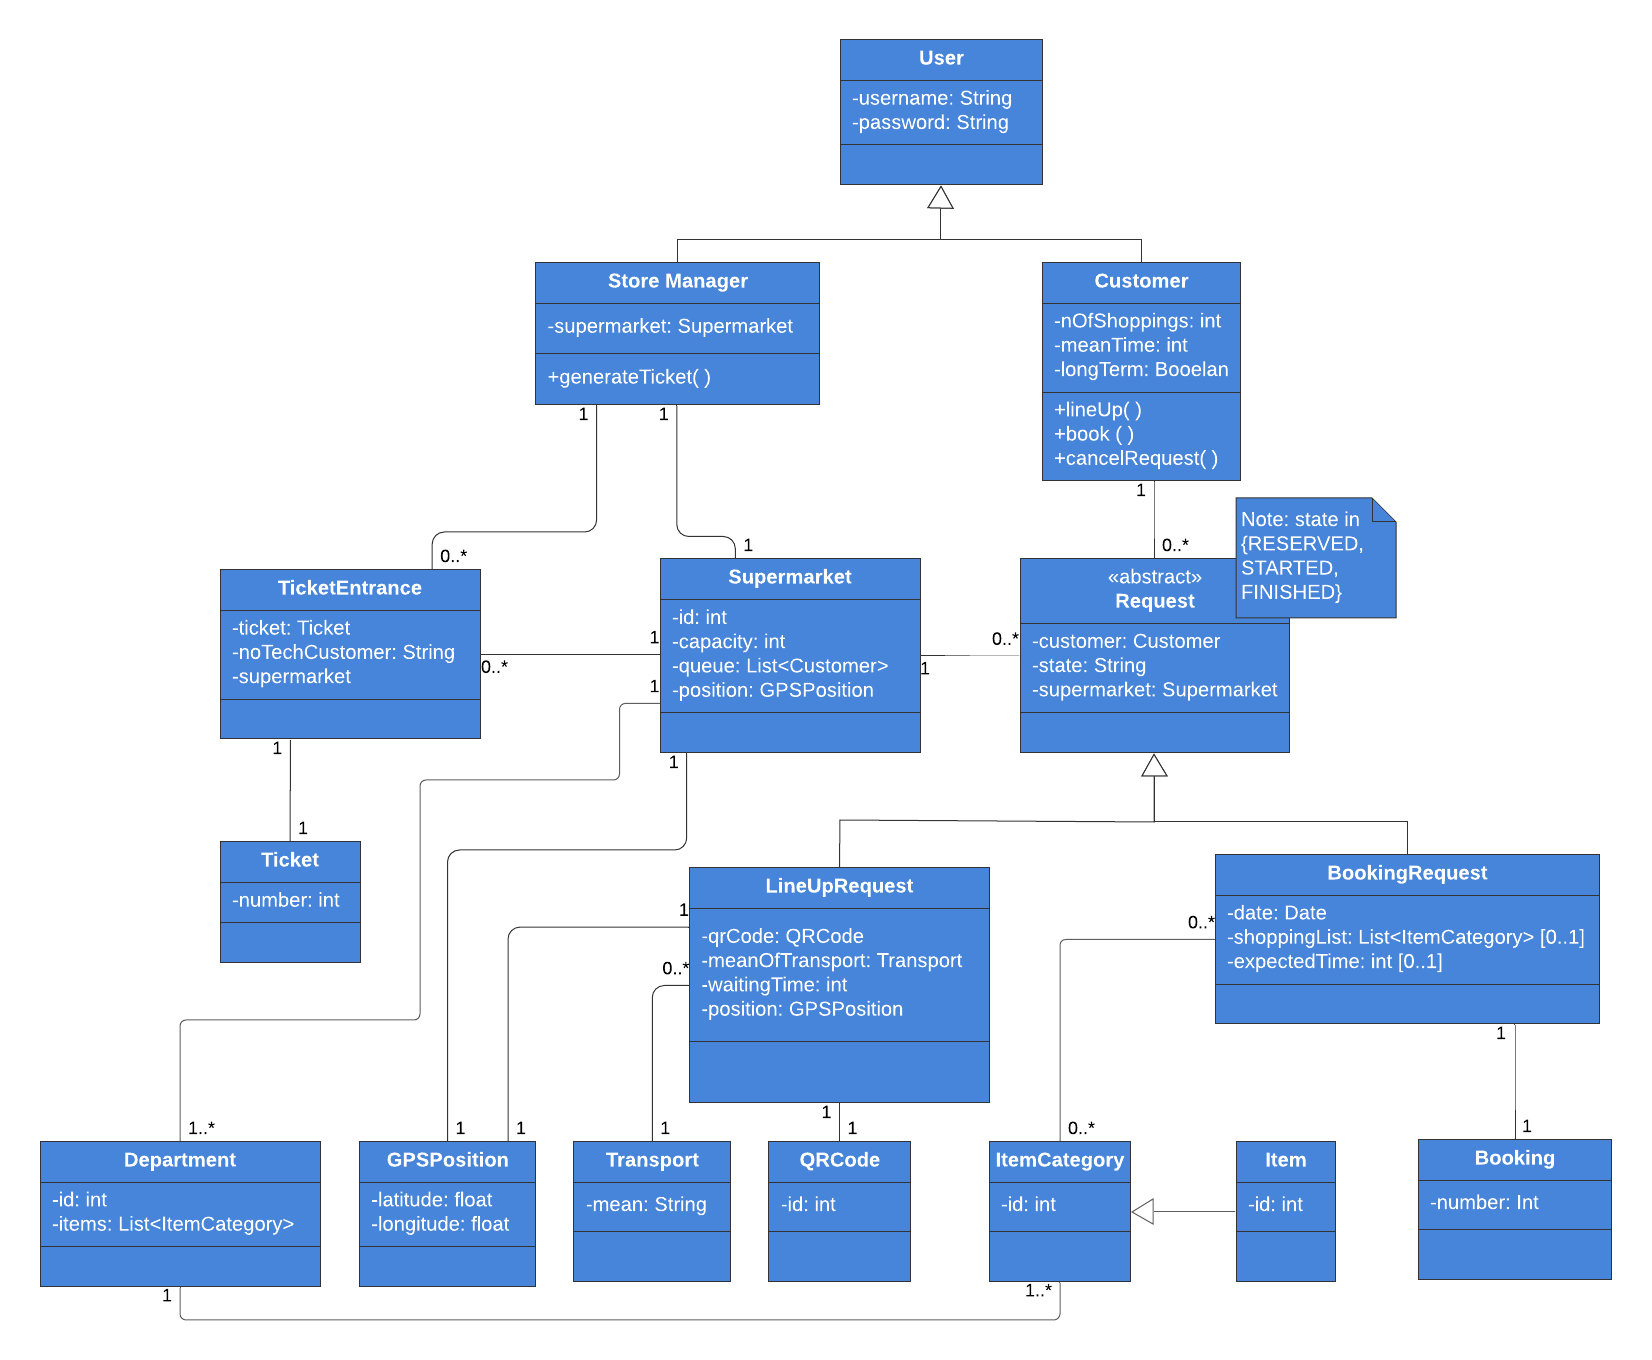
\includegraphics[scale=0.75]{./ClassDiagramDD}}
\caption{Class Diagram}
\end{figure}